\section{Gauß Law in Minkowski Space}
\label{sec:Apdx_GaußLawMinkowski}

From the Gauß law in Euclidean space
\begin{equation}
    \int_\Omega\dt\Omega\,\vec{\partial}\cdot\vec{J}=\int_{\partial_\Omega}\dt\vec{\sigma}\cdot \vec{J}\,,
    \label{eq:GaußLawEuclidean}
\end{equation}
where ${\vec{\partial}\cdot\vec{J}\equiv\sum \partial_i J^i}$ is the divergence of $\vec{J}$, we wish to derive an analogous statement in Minkowski space, considering the differences in the metric signature. For simplicity, let $\Omega$ be the region depicted in \ref{fig:GaußMinkowksi_Example} in a 1+1-dimensional spacetime with cartesian coordinates $(t,x)$. Assume the only relevant boundaries are parametrized by $x=x_\star=\const$ and $t=t_\star=\const$ and contributions at all other boundaries vanish.\\
\debugbox{
\begin{minipage}{\linewidth}
    \centering
    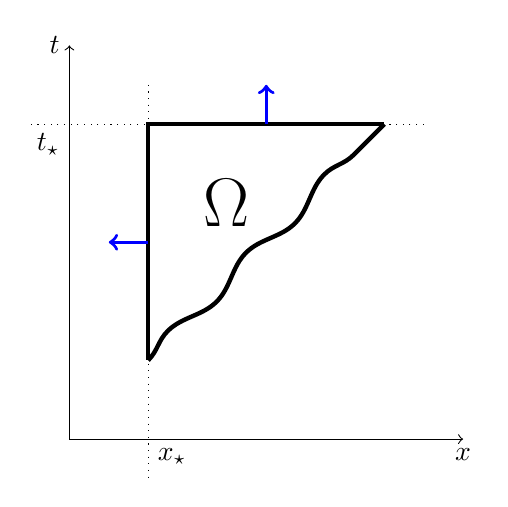
\begin{tikzpicture}
        \draw[->] (0,0) -- (5,0) node[below]{$x$};
        \draw[->] (0,0) -- (0,5) node[left]{$t$};

        \draw[ultra thick] (4,4) -- (1,4) -- (1,1);
        \draw[dotted] (4.5,4) -- (-0.5,4);
        \draw[dotted] (1,4.5) -- (1,-0.5);
        \draw[decorate,decoration={snake,segment length=40,post length=0},ultra thick] (1,1) -- (4,4);

        \draw[very thick, ->, blue] (1,2.5) -- (0.5,2.5);
        \draw[very thick, ->, blue] (2.5,4) -- (2.5,4.5);

        \node at (2,3) {\Huge$\Omega$};
        \node[anchor=north west] at (1,0) {$x_{\star}$};
        \node[anchor=north east] at (0,4) {$t_{\star}$};
    \end{tikzpicture}
    \captionof{figure}{Region of 1+1-dimensional spacetime with outwards oriented normal vectors ${\propto\dt\vec{\sigma}}$ (blue).}
    \label{fig:GaußMinkowksi_Example}
\end{minipage}
}

Denote $J^\mu\equiv\vec{J}\equiv(J^t,J^x)$ and calculate.
\begin{subequations}
    \begin{align}
        \int_\Omega\dt\Omega\,\partial_\mu J^\mu&=\int_\Omega\dt\Omega(\partial_tJ^t+\partial_xJ^x)\\
        \intertext{\dots apply \ref{eq:GaußLawEuclidean}\dots}
        &=\int_{\partial\Omega}\dt\vec{\sigma}\cdot \vec{J}\\
        &=\int_{t=t_\star}\dt x\begin{pmatrix}
            1\\0
        \end{pmatrix}^T\begin{pmatrix}
            J^t\\J^x
        \end{pmatrix}
        +\int_{x=x^\star}\dt t\begin{pmatrix}
            0\\-1
        \end{pmatrix}^T\begin{pmatrix}
            J^t\\J^x
        \end{pmatrix}\\
        &=-\int_{t=t_\star}\dt x\begin{pmatrix}
            1\\0
        \end{pmatrix}^T\begin{pmatrix}
        -1&0\\0&1
        \end{pmatrix}\begin{pmatrix}
            J^t\\J^x
        \end{pmatrix}
        +\int_{x=x^\star}\dt t\begin{pmatrix}
            0\\-1
        \end{pmatrix}^T\begin{pmatrix}
            -1&0\\0&1
        \end{pmatrix}\begin{pmatrix}
            J^t\\J^x
        \end{pmatrix}
    \end{align}
\end{subequations}
which can be generalized to
\begin{equation}
    \int_\Omega\dt\Omega\,\partial_\mu J^\mu=-\Big(\int_{\partial\Omega,\text{spacelike}}\dt\sigma^\mu\eta_{\mu\nu}J^\nu-\int_{\partial\Omega,\text{timelike}}\dt\sigma^\mu\eta_{\mu\nu}J^\nu\Big)
\end{equation}
Thus, unlike in the purely Euclidean case, there is a relative "-"-sign between contributions from spacelike and timelike boundaries in Minkowski space, as well as an overall "-"-sign due to the metric convention.